\documentclass[12pt,a4paper,oneside,titlepage,onecolumn]{article}


% Para Português
\usepackage[utf8]{inputenc}
\usepackage[brazil]{babel}

% Insert pages from PDFs
\usepackage{pdfpages}
% Generate filler text
\usepackage{lipsum}
% Control the font size
\usepackage{anyfontsize}
% For inserting figures
\usepackage{graphicx}
% Mathematical Symbols and fonts
\usepackage{amssymb,amsmath}
% Bibliography citations
\usepackage[round]{natbib}

% Set margins
\usepackage{setspace}
\usepackage[a4paper]{geometry}
\geometry{verbose,tmargin=3cm,bmargin=3cm,lmargin=3cm,rmargin=3cm}

% Metadata and hyperlinks
\usepackage[pdftex,colorlinks=true]{hyperref}
\newcommand{\Title}{Memorial de Leonardo Uieda}
\hypersetup{
    pdftitle={\Title},
    pdfauthor={Leonardo Uieda},
    pdfsubject={Memorial para concurso de Professor Doutor na USP},
    pdfcreator={pdfTeX},
    allcolors=black,
}

% Make the fancy header
\usepackage{fancyhdr}
\pagestyle{fancy}
\lhead{MEMORIAL DE LEONARDO UIEDA}
\cfoot{\thepage}


\begin{document}

\begin{titlepage}

\begin{center}



{\LARGE \textbf{MEMORIAL}}
\\[3cm]


{\large LEONARDO UIEDA}
\\[3cm]
\vfill

% Bottom of the page
{\large São Paulo
\\[0.2cm]
2009}


\end{center}

\end{titlepage}



\begin{titlepage}
    \begin{center}
        \hspace{\fill}
        \\[6cm]

        {\Huge \textbf{Memorial}}
        \\[3cm]

        {\Large Leonardo Uieda}
        \\[3cm]

        \begin{flushright}
        \parbox{9cm}{\large
            Apresentado para concurso público de títulos e provas para cargo de
            Professor Doutor junto ao Departamento de Geofísica do Instituto de
            Astronomia, Geofísica e Ciências Atmosféricas da Universidade de
            São Paulo.
        }
        \end{flushright}
        \vfill

        {\large 2017}
    \end{center}
\end{titlepage}



\pagenumbering{roman}
\singlespacing

\thispagestyle{plain}
\tableofcontents
\newpage

\pagenumbering{arabic}
\onehalfspacing

\thispagestyle{plain}
\section{Introdução}

Resumo dos títulos e entrada na UERJ.

Ciência aberta e código no github e site (coisas na net).

Papers: quantos, colaborações.

Trabalhos em congressos: quantos, colaborações, quais congressos.

Como vou organizar esse memorial.
Divido em três temas.

O primeiro, Software, está por trás de todo meu trabalho nos demais.
Desenvolvo esses programas para facilitar minha pesquisa, complementar e
fortalecer minhas técnicas de ensino e como forma de conectar com a comunidade
da geofísica nacional e internacional.

Tive dificuldade em elaborar uma organização coerente para esses temas.
O desenvolvimento de software esteve presente ao longo de toda minha carreira.
Uma ordem cronológica seria muito confuso por que os temas se misturam contribuem entre si.

Software

Pesquisa

Ensino

\citet{uieda2016a}

\lipsum[1-10]

\newpage

\thispagestyle{plain}
\section{Software}


\subsection{Formação}

Meu primeiro contato com a programação foi através da disciplina
``Introdução à Computação para Ciências Exatas e Tecnologia''
que cursei em 2004 durante meu primeiro semestre na USP.
Antes disso, eu não tinha conhecimento algum de como programas de computador
são feitos ou que qualquer um poderia criar o seu próprio programa.
Aprendi os conceitos básicos da linguagem de programação C.
Porem, não acalcei um nível suficientemente avançado para enxergar aplicações
imediatas da programação nas demais disciplinas do curso de geofísica.

Busquei aprender mais sobre a linguagem C através da disciplina optativa
``Computação para Geofísicos''.
Nela desenvolvi aplicações diretas à geofísica como o cálculo do International
Geomagnetic Reference Field (IGRF) a partir dos coeficientes de harmônicos
esféricos e o método de \citet{talwani1959} para modelagem direta na
gravimetria.
O código que criei para a disciplina foi utilizado anos depois como base
para a implementação do método de \citet{talwani1959} no programa
\textit{Fatiando a
Terra}\footnote{\url{www.fatiando.org/v0.5/api/gravmag.talwani.html}}.
Essas aplicações me mostraram o enorme poder da programação no aprendizado de
conceitos complexos da geofísica e matemática.
Ao criar uma implementação computacional de um método, o aluno é levado a
considerar detalhes e fazer perguntas que pode não ter notado ao estudar a
teoria.
Além disso, também é capaz de explorar as possibilidades e os limites de uma
teoria de forma dinâmica e independente.
Não exagero quando afirmo que ter cursado a disciplina ``Computação para
Geofísicos'' foi crucial para o resto de minha carreira.

Nos anos seguintes comecei a estudar a programação nas horas vagas e a aplicar
à geofísica o que estava aprendendo.
Implementei a Transformada Discreta de Fourier\footnote{Disponível em
\url{https://github.com/leouieda/dft-in-c}} para estudar para a disciplina
``Processamento de Sinais Digitais''.
Utilizei minha implementação do método de otimização Ant Colony Optimization
\citep{socha2008} para realizar uma inversão das velocidades de grupo de ondas
Love\footnote{Disponível em \url{https://github.com/leouieda/love-aco-inv}}
para a disciplina ``Teoria de Ondas Sísmicas e Estrutura da Terra''.
Para as disciplinas de geodésia que cursei durante meu intercâmbio na York
University, implementei ajustes de redes gravimétricas, mudança de sistemas de
coordenadas geográficas, entre outros.
Aprendi as linguagens de programação C++, Java e Python.
Cursei a disciplina optativa ``Princípios de Desenvolvimento de Algoritmos''
onde aprendi os conceitos que possibilitaram os avanços que obtive em
\citet{tesseroids}.

Meu projeto de conclusão de curso foi o tesseroids (ver a seguir).


Conheci o Software Carpentry em 2008 e tudo mudou.
Descobri o quanto não sabia sobre coisas básicas na indústria.
Principalmente testes e controle de versão.
Comecei a prender sobre essas tecnologias e utilizá-las no meu dia a dia.

Na pós continuei com essa abordagem de implementar tudo.
Comecei a construir o Fatiando.
Muitas coisas se tornaram parte do Fatiando.
Na geotermia implementei a variação climática
http://www.fatiando.org/v0.5/api/geothermal.climsig.html
Na gravimetria implementei as modelagens diretas, etc.

Fui aprendendo com a experiência e melhorando meu Python.

Melhores jeitos de testar.

Como tornar o código mais rápido.

Como utilizar paralelismo de forma básica.

Aprendi os desafios da distribuição de software para múltiplos sistemas
operacionais.

Como criar documentação para um projeto.

Principalmente como facilitar e encorajar colaboradores novos.

Esse último ainda estou aprimorando.







\subsection{Tesseroids}

Em 2007 iniciei um estágio de iniciação científica com a Profa. Dra. Naomi
Ussami.
Meu projeto era parte de uma colaboração com a Profa. Dra. Carla Braitenberg da
University of Trieste, Itália.
O objetivo dessa colaboração era preparar a comunidade científica para lidar
com os dados de gradiometria gravimétrica que seriam coletados pelo satélite
GOCE (Gravity field and steady-state Ocean Circulation Explorer).
Minha parte nesse projeto era desenvolver um programa para a modelagem direta
dos dados utilizando tesseroides (prismas esféricos).

Tesseroids e Colaboração com Carla
AGU 2010
GOCE 2011
Utilizações


\subsection{Fatiando a Terra}

Fatiando
Scipy 2013 e 2014
Boletim sbgf
Palestra USP, ON e UH
Utilizações

Na versão 0.3 de 2014, éramos somente 5 pessoas, todos amigos de faculdade.

Em 2017 a futura versão 0.6 conta com 13 pessoas.


\subsection{GMT/Python}

GMT
Scipy  2017

\newpage

\thispagestyle{plain}
\section{Pesquisa}

Minha pesquisa se concentra na área de problemas inversos em métodos
potenciais.
Geralmente, meus trabalhos são avanços metodológicos e são acompanhados por
um código fonte que os implementa.
Como mencionei no capítulo \ref{software}, acredito que o código fonte que
acompanha uma publicação é tão importante quanto a descrição de sua
metodologia.
Muitas vezes é impossível reproduzir os resultados de um trabalho
sem ter acesso ao software que os gerou.
Logo, é crucial que o código esteja disponível para ser revisado pela
comunidade científica.
Para tanto, disponibilizo o código e dados (à medida do possível) necessários
para reproduzir os resultados de meus trabalhos como primeiro autor.
Cada trabalho é acompanhado de um repositório na página do Grupo de Pesquisa em
Problemas Inversos em Geofísica (\url{https://github.com/pinga-lab}).
Os repositórios contém o código fonte que implementa a metodologia, realiza os
testes com dados sintéticos e produz as figuras para o artigo.
Ultimamente, torno público um repositório no momento da submissão do respectivo
artigo para publicação.
Dessa forma, os revisores tem acesso ao conteúdo total de meus trabalhos e
podem se certificarem de que meus resultados estão corretos.
Cada repositório também é arquivado permanentemente e recebe um Digital Object
Identifier (DOI) através de serviços como Zenodo (\url{http://zenodo.org}) e
figshare (\url{https://figshare.com}).

A seguir, apresento reflexões sobre os aspectos de minha formação que me
levaram a essa área de pesquisa e sobre os diferentes trabalhos que formam
minha produção acadêmica.


\subsection{Formação}

Desde o início da graduação me senti intrigado pelos métodos de inversão.
Sempre ouvia de alunos veteranos, ou até mesmo de professores, que esse era um
assunto extremamente complexo.
Conhecendo minha personalidade, creio que meu interesse inicial sobre o assunto
era puramente devido ao desafio.
Por sorte, a disciplina que forma a base do conhecimento de problemas inversos,
a álgebra linear, também foi um tema que despertou meu interesse.
Por outro lado, devo confessar que, a princípio, os métodos potenciais não me
interessaram tanto quando a inversão.
Minha primeira impressão da gravimetria e magnetometria foi que eram métodos
simples.
Porém, terminei minha primeira disciplina sobre o assunto completamente confuso
e com mais dúvidas do que tinha antes de cursá-la.
Hoje percebo que essas são características de um assunto complexo e
interessante e de uma aula de qualidade.

Fiz minha primeira iniciação científica no laboratório de paleomagnetismo com
bolsa da FAPESP e orientação do Prof. Manoel S. D'Agrella Filho.
Ao final do período de um ano da bolsa, decidi não continuar nessa área.
Em seguida, busquei outro projeto que unisse a geofísica
com meu interesse pela programação.
Em 2007, iniciei o projeto sob orientação da
Profa. Naomi Ussami que resultou no software \textit{Tesseroids}.

Em 2008, realizei um programa de intercâmbio de 10 meses na York University,
Canadá.
Parte do motivo para essa escolha é a excelência do país nas áreas de
gravimetria e geodésia.
Lá, cursei disciplinas sobre geodésia física, gravimetria e ajuste de redes
através do método dos mínimos quadrados.

Em 2010, ingressei no Mestrado em Geofísica do Observatório Nacional sob
orientação da Profa. Valéria C. F. Barbosa.
Meu projeto era criar um método de inversão 3D de dados de gradiometria
gravimétrica, tema que contava com atenção internacional e era pioneiro no
cenário nacional.
Nesse ponto, percebi que as disciplinas cursadas na York me forneceram a base
necessária para compreender a inversão e a gravimetria com muito mais
facilidade.
Aprendi com a Profa. Valéria
as diferentes vertentes e sutilezas da inversão,
a arte da elaboração de artigo científico
e sua ética profissional impecável.
Também devo muito do meu aprendizado durante a pós-graduação às longas
conversas e debates com meu amigo Vanderlei C. Oliveira Jr. (atualmente
pesquisador do Observatório Nacional).



\subsection{Modelagem direta de campos gravitacionais com tesseroides}

Comecei a desenvolver esse tema durante minha iniciação científica com a
Profa. Naomi de 2007 a 2009.
A princípio, meu trabalho simplesmente aprender a metodologia de
\citet{wild-pfeiffer2008} e transformá-la em um programa de computador.
Apresentei meu primeiro trabalho em um evento internacional sobre os resultados
de meu trabalho de conclusão de curso:

\begin{displayquote}
    UIEDA, L.; USSAMI, N.; BRAITENBERG, C. Computation of the gravity
    gradient tensor due to topographic masses using tesseroids. In: AGU Meeting
    of the Americas, 2010.\footnote{Apresentação disponível em
    \url{http://www.leouieda.com/talks/agu2010.html}}
\end{displayquote}

Retomei esse projeto em 2011 durante minha estadia em Trieste com a Profa.
Braitenberg para atualizar o software e a metodologia para o cálculo dos campos
gravitacionais de um tesseroide (prisma esférico).
Utilizei as equações otimizadas de \citet{grombein2013} para eliminar
as singularidades presentes na formulação de \citet{wild-pfeiffer2008}.
Também desenvolvi um método de discretização adaptativa dos tesseroides para
garantir a acurácia da integração numérica com a Quadratura Gauss-Legendre.
Sem meu conhecimento, um algoritmo similar \citep{li2011} havia sido publicado
no mesmo período em que estava em Trieste, inviabilizando a nossa publicação do
método.
Ainda em Trieste, busquei caracterizar o erro numérico envolvido
nos cálculos para melhorar controlar a discretização adaptativa.
Publiquei meus esforços com o software \textit{Tesseroids} e os resultados da
análise do erro da quadratura nos anais do 4th International GOCE User
Workshop:

\begin{displayquote}
    UIEDA, L.; BOMFIM, E. P.; BRAITENBERG, C.; MOLINA, E. C. Optimal
    forward calculation method of the Marussi tensor due to a geologic
    structure at GOCE height. In: 4th International GOCE User Workshop,
    2011.\footnote{Pôster e texto disponíveis em
    \url{http://www.leouieda.com/posters/goce2011.html}}
\end{displayquote}

Para minha tese de doutorado, iria utilizar a modelagem direta com tesseroides
para desenvolver um método de inversão em coordenadas esféricas.
Porém, para que a inversão seja correta é necessário que a modelagem direta
seja o mais precisa possível.
Logo, continuei com o desenvolvimento do algoritmo de discretização adaptativa
e com os experimentos para caracterizar o erro da quadratura.
Após diversas tentativas frustadas, cheguei aos resultados apresentados no
artigo:

\begin{displayquote}
    UIEDA, L; BARBOSA, V. C. F.; BRAITENBERG, C. Tesseroids:
    Forward-modeling gravitational fields in spherical coordinates. Geophysics,
    v. 81, p. F41-F48, 2016.\footnote{Código fonte disponível em
    \url{https://github.com/pinga-lab/paper-tesseroids}}
\end{displayquote}

Neste trabalho, aprimoramos o algoritmo de discretização adaptativa proposto
por \citet{li2011}.
Também determinamos empiricamente valores para o parâmetro
\textit{distance-size ratio}, que controla a discretização adaptativa,
para manter o erro de integração abaixo de $0.1\%$.

Os trabalhos relacionados à essa metodologia estão entre meus trabalhos mais
citados.
Acredito que isso é devido em parte à disponibilização do software
\textit{Tesseroids} que implementa essa metodologia.
Outro fruto dessa pesquisa é minha coorientação da tese de doutorado do aluno
Santiago Soler com o Prof. Dr. Mario Ernesto Gimenez da Universidad Nacional de
San Juan, Argentina.
A tese de Santiago dará continuidade à modelagem direta com tesseroides,
expandindo a formulação para incluir tesseroides com distribuições internas de
densidades variáveis.


\subsection{Inversão 3D utilizando o método de plantação}

Meu projeto de mestrado era desenvolver um método de inversão 3D para dados de
gradiometria gravimétrica.
Um dos desafios enfrentados nessa área é o aumento significativo do número de
dados em uma aquisição gradiométrica comparados com uma aquisição
aerogravimétrica.
Esse aumento tornava a inversão impossível de ser executada nos computadores
que tínhamos disponíveis no Observatório Nacional.

Minha ideia inicial para o método de inversão surgiu durante uma conversa com o
Prof. Dr. João B. C. Silva da Universidade Federal do Pará.
No momento, ele se encontrava no Rio de Janeiro para participar de uma banca de
mestrado.
Durante a conversa, o Prof. João mencionou o trabalho de \citet{rene} como um
exemplo de uma metodologia diferente e pouco reconhecida pela comunidade
científica.
\citet{rene} propôs um método de inversão 2D de dados gravimétricos na qual a
solução cresce em torno de alguns elementos nucleares chamados de ``sementes''.
O que despertou meu interesse nesse trabalho foi o viés computacional do método
proposto, ao invés da abordagem matemática clássica.
Ao estudá-lo, percebi que poderia ser adaptado e aprimorado para o
caso 3D e dados de gradiometria gravimétrica.
Minhas modificações incluem a introdução da função de regularização de
compacidade de \citet{silvadias2009},
um termo de normalização para as funções do ajuste
e a avaliação parcial da matriz de sensibilidade.
Esta última modificação é a que possibilita a inversão de conjuntos grandes de
dados com poucos recursos computacionais.

Apresentei este novo método, denominado ``método de plantação'',  nos
congressos internacionais
73rd EAGE Conference and Exhibition incorporating SPE EUROPEC,
SEG International Exposition and Eighty-First Annual Meeting,
12th International Congress of the Brazilian Geophysical Society,
e
International Symposium on Gravity, Geoid and Height Systems.
Fui premiado com auxílio financeiro da Near Surface Geophysics Section (NSGS)
da SEG para participar do SEG Annual Meeting.
Também obtive o auxílio PACE Student Travel Grant para participar do 73rd EAGE
Conference and Exhibition.

Publiquei trabalhos completos nos anais de 3 desses eventos:

\begin{displayquote}
    UIEDA, L.; BARBOSA, V. C. F. 3D gravity Gradient Inversion by Planting
    Density Anomalies. In: 73rd EAGE Conference and Exhibition incorporating
    SPE EUROPEC, 2011, Vienna. v. 1.\footnote{Pôster e código fonte:
    \url{http://www.leouieda.com/posters/eage2011.html}}
\end{displayquote}

\begin{displayquote}
    UIEDA, L.; BARBOSA, V. C. F. Robust 3D gravity gradient
    inversion by planting anomalous densities. In: SEG International Exposition
    and Eighty-First Annual Meeting, 2011, San Antonio. p.
    820-824.\footnote{Apresentação e código fonte:
    \url{http://www.leouieda.com/talks/seg2011.html}}
\end{displayquote}

\begin{displayquote}
    UIEDA, L.; BARBOSA, V. C. F. 3D gravity inversion by planting
    anomalous densities. In: 12th International Congress of the Brazilian
    Geophysical Society, Rio de Janeiro, Brazil,
    2011.\footnote{Apresentação e código fonte:
    \url{http://www.leouieda.com/talks/sbgf2011.html}}
\end{displayquote}

Subsequentemente, publiquei meu primeiro artigo em periódico:

\begin{displayquote}
    UIEDA, L.; BARBOSA, V. C. F. Robust 3D gravity gradient inversion by
    planting anomalous densities. Geophysics, v. 77, p. G55-G66,
    2012.\footnote{Código fonte disponível em
    \url{https://github.com/pinga-lab/paper-planting-densities}}
\end{displayquote}

O próximo passo no desenvolvimento desse método veio quando, ao ler novamente o
trabalho original de \citet{rene}, percebi as enormes vantagens da utilização
da função ``shape-of-anomaly''.
Essa função é definida e utilizada no trabalho de 1986.
Porém, acredito que René não explorou todas suas implicações para a inversão.
Ao utilizá-la em meu método de plantação, percebi que era capaz de obter
resultados melhores utilizando menos elementos nucleares (as ``sementes'' da
inversão).
Apresentei estes resultados e uma análise do motivo de seu sucesso no congresso
SEG International Exposition and Eighty-Second Annual Meeting,
acompanhado da publicação nos anais do evento:

\begin{displayquote}
    UIEDA, L.; BARBOSA, V. C. F. Use of the shape-of-anomaly data
    misfit in 3D inversion by planting anomalous densities. In: SEG Technical
    Program Expanded Abstracts 2012.\footnote{Apresentação e código fonte:
    \url{http://www.leouieda.com/talks/seg2012.html}}
\end{displayquote}


Durante meu doutorado, adaptei este método para a inversão de dados de anomalia
magnética de campo total com resultados insatisfatórios.
Os resultados da inversão se mostraram extremamente sensíveis à direção de
magnetização total assumida para o alvo.
Não dei continuidade com esse trabalho pois o foco de minha tese havia mudado
para a inversões em escala regional.
Apresentei meus resultados no evento AGU Meeting of the Americas de 2013:

\begin{displayquote}
    UIEDA, L.; BARBOSA, V. C. F. 3D magnetic inversion by planting anomalous
    densities. In: AGU Meeting of the Americas, 2013,
    Cancun.\footnote{Apresentação e código fonte:
    \url{http://www.leouieda.com/talks/agu-cancun2013.html}}
\end{displayquote}

Em seguida, adaptei o método de plantação para utilizar tesseroides ao invés de
prismas retangulares retos.
Dessa forma, poderia realizar a inversão em coordenadas esféricas e em escala
regional.
No entanto, o método de plantação assume que os alvos da inversão são corpos
contínuos e com contraste de densidade abrupto em relação às estruturas
encaixantes.
Embora o método funcione em testes com dados sintéticos,
tive dificuldade de encontrar situações reais onde o método se aplicaria.
Apresentei esses resultados no EGU General Assembly de 2014:

\begin{displayquote}
    UIEDA, L.; BARBOSA, V. C. F. Gravity inversion in spherical
    coordinates using tesseroids. In: EGU General Assembly 2014.
    EGU2014-10898-1.\footnote{Apresentação e código fonte:
    \url{http://www.leouieda.com/talks/egu2014.html}}
\end{displayquote}


O método de plantação foi utilizado na tese de doutorado de Dionísio U. Carlos,
que na época era aluno da Profa. Valéria, para modelar dados de gradiometria do
Quadrilátero Ferrífero.
Dessa colaboração com o Dionísio foram publicados 3 trabalhos completos em
anais de eventos e 2 artigos em periódicos internacionais:

\begin{displayquote}
    CARLOS, D. U.; BARBOSA, V. C. F.; UIEDA, L.; BRAGA, M. A. Inversão de
    dados de aerogradiometria gravimétrica 3D-FTG aplicada a exploração mineral
    na região do Quadrilátero Ferrífero. In: 12th International Congress of the
    Brazilian Geophysical Society, 2011.
\end{displayquote}

\begin{displayquote}
    CARLOS, D. U.; UIEDA, L.; BARBOSA, V. C. F.; BRAGA,
    M. A.; GOMES, A. A. S. In-depth imaging of an iron
    orebody from Quadrilatero Ferrifero using 3D gravity gradient inversion.
    In: SEG International Exposition and Eighty-First Annual Meeting, 2011.
\end{displayquote}

\begin{displayquote}
    CARLOS, D. U,; UIEDA, L.; LI, Y.; BARBOSA, V.
    C. F.; BRAGA, M. A. ; ANGELI, G.; PERES, G. Iron ore
    interpretation using gravity-gradient inversions in the Carajás, Brazil.
    In: SEG Technical Program Expanded Abstracts 2012.
\end{displayquote}

\begin{displayquote}
    CARLOS, D. U.; UIEDA, L.; BARBOSA, V. C. F. Imaging
    iron ore from the Quadrilátero Ferrífero (Brazil) using geophysical
    inversion and drill hole data. Ore Geology Reviews, v. 61, p. 268-285,
    2014.
\end{displayquote}

\begin{displayquote}
    CARLOS, D. U.; UIEDA, L.; BARBOSA, V. C. F. How two
    gravity-gradient inversion methods can be used to reveal different geologic
    features of ore deposit - A case study from the Quadrilátero Ferrífero
    (Brazil). Journal of Applied Geophysics, v. 130, p. 153-168, 2016.
\end{displayquote}


O método de plantação \citep{seed} é meu trabalho mais citado\footnote{Segundo
a base Google Scholar:
\url{https://scholar.google.com.br/citations?user=qfmPrUEAAAAJ&hl=en}} e o que
me rendeu o maior número de publicações.
Este trabalho marcou minha iniciação
à apresentação de trabalhos em congressos no exterior e
à escrita e publicação de artigos científicos.
Também serviu como um primeiro experimento das possibilidades de tornar
pesquisa mais transparente, acessível e reprodutível.


\subsection{Inversão 3D em coordenadas esféricas}


Começou com o último trabalho da sementes (EGU 2014).
Inversão da Moho


\subsection{Camada Equivalente}

A técnica da camada equivalente é utilizada para o processamento de dados de
métodos potenciais.
Suas aplicações incluem a interpolação de dados, continuação para cima, redução
ao polo, remoção de ruídos aleatórios e cálculo de derivadas.
A camada equivalente é aplicada em dois passos:
primeiro, estimamos os coeficientes de uma série de funções harmônicas que
melhor ajustam os dados observados;
segundo, utilizamos os coeficientes estimados para realizar a transformação
desejada através da modelagem direta.
É comum utilizar como as funções harmônicas o efeito de uma malha regular de
fontes pontuais.
Dessa forma, os coeficientes estimados possuem significado físico.
Por exemplo, no caso da gravimetria os coeficientes representam as densidades
de massas pontuais.
A camada equivalente é capaz de operar em dados distribuídos de forma irregular
e é geralmente mais estável que métodos que utilizam a Transformada de Fourier.
Porém, o primeiro passo para sua aplicação é uma inversão, o que a torna
computacionalmente custosa.

Das muitas conversas que tive com o Vanderlei durante a pós-graduação,
surgiu a ideia de parametrizar a camada equivalente utilizando polinômios
bidimensionais no lugar de fontes pontuais.
A camada seria dividida em janelas e a distribuição de propriedades físicas
dentro de cada janela seria representada por um polinômio.
Essa parametrização nos possibilitaria estimar os coeficientes desses
polinômios ao invés de estimar os valores de propriedade física de cada fonte
pontual.
Esta mudança reduz drasticamente o número de parâmetros a serem estimados na
inversão.

Essa ideia foi executada pelo Vanderlei e se tornou parte de sua tese de
doutorado.
Publicamos o método desenvolvido na revista \textit{Geophysics} em 2013:

\begin{displayquote}
    OLIVEIRA Jr., V. C.; BARBOSA,  V. C. F.; UIEDA, L. Polynomial equivalent
    layer. GEOPHYSICS, 78(1), G1-G13, 2013.
\end{displayquote}


\subsection{Estimação da direção de magnetização}

magdir


\subsection{Deconvolução de Euler}

Colaboração com Figura.


\subsection{Tutoriais sobre geofísica}

Tutorial Euler
Tutorial NMO

\newpage

\thispagestyle{plain}
\section{Ensino}

Posição sobre ensino e material didático.
Experiência e entrada na UERJ.

\subsection{Minicursos}

\subsubsection{Tópicos de inversão em geofísica (IAG/USP)}

\subsubsection{Tópicos de inversão em geofísica (UnB)}

\subsubsection{Python como uma ferramenta numérica em Ciências da Terra (IAG/USP)}

Python como uma ferramenta numérica em Ciências da Terra: Uma
nova abordagem de programação

\subsubsection{Python para Geologia (UERJ)}

\subsubsection{Introduction to Python Workshop (University of Hawaii)}


\subsection{Disciplinas de graduação na UERJ}

Entrada UERJ

Disciplinas

Homenagem


\subsection{Orientações, coorientações e treinamento}

Orientação do Vinícius e Fernanda.

Santiago

Qualitec e Victor

\newpage

\thispagestyle{plain}
\section{Conclusão}

\lipsum[1-3]

\newpage

\appendix

\thispagestyle{plain}
\section{Curriculum Vitae}


\subsection{Formação acadêmica}
%%%%%%%%%%%%%%%%%%%%%%%%%%%%%%%%%%%%%%%%%%%%%%%%%%%%%%%%%%%%%%%%%%%%%%%%%%%%%%%

\begin{itemize}
    \item \textbf{Pós-doutorado} (02/2017 - Presente),
        University of Hawaii, Honolulu, E.U.A.
        Projeto: Expansion of the Generic Mapping Tools (GMT) to the Python
        programming language.
        Supervisor: Paul Wessel.
        Bolsista da National Science Foundation (NSF), E.U.A.
    \item \textbf{Doutorado em Geofísica} (11/2011 - 04/2016),
        Observatório Nacional, Rio de Janeiro, Brasil.
        Tese: Modelagem direta e inversão de campos gravitacionais em
        coordenadas esféricas.
        Orientadora: Valéria Cristina Ferreira Barbosa.
        Bolsista da Coordenação de Aperfeiçoamento de Pessoal de Nível
        Superior (CAPES).
    \item \textbf{Mestrado em Geofísica} (02/2010 - 10/2011),
        Observatório Nacional, Rio de Janeiro, Brasil.
        Dissertação: Robust 3D gravity gradient inversion by planting anomalous
        densities.
        Orientadora: Valéria Cristina Ferreira Barbosa.
        Bolsista da Coordenação de Aperfeiçoamento de Pessoal de Nível
        Superior (CAPES).
    \item \textbf{Intercâmbio Internacional} (08/2008 - 05/2009),
        York University, Toronto, Canadá.
    \item \textbf{Bacharelado em Geofísica} (02/2004 - 12/2009),
        Universidade de São Paulo, São Paulo, Brasil.
        Trabalho de conclusão: Cálculo do tensor gradiente gravimétrico
        utilizando tesseroides.
        Orientadora: Naomi Ussami.
        Bolsista da Sociedade Brasileira de Geofísica (SBGf).
\end{itemize}


\subsection{Atuação profissional}
%%%%%%%%%%%%%%%%%%%%%%%%%%%%%%%%%%%%%%%%%%%%%%%%%%%%%%%%%%%%%%%%%%%%%%%%%%%%%%%

\begin{itemize}
    \item \textbf{Professor Assistente} (02/2014 - Presente), regime de 40
        horas semanais,
        Universidade do Estado do Rio de Janeiro, Rio de Janeiro, Brasil.
        Coordenador do Laboratório de Geofísica de Exploração. Responsável
        pelas disciplinas Geofísica 1, Geofísica 2 e Matemática Especial I.
\end{itemize}


\subsection{Coordenação de Projetos}
%%%%%%%%%%%%%%%%%%%%%%%%%%%%%%%%%%%%%%%%%%%%%%%%%%%%%%%%%%%%%%%%%%%%%%%%%%%%%%%

\begin{itemize}
    \item \textbf{Projeto Qualitec 2014 para bolsista de Nível Superior}
        (10/2014 - Presente).
        Bolsa para treinamento de um técnico de nível superior para o
        Laboratório de Geofísica de Exploração (LAGEX).
        Financiador: Universidade do Estado do Rio de Janeiro.
\end{itemize}


\subsection{Revisor de periódicos}
%%%%%%%%%%%%%%%%%%%%%%%%%%%%%%%%%%%%%%%%%%%%%%%%%%%%%%%%%%%%%%%%%%%%%%%%%%%%%%%

\begin{itemize}
    \item Computers \& Geosciences - Início em 2011.
    \item Geophysics - Início em 2013.
    \item Central European Journal of Geosciences (Open Geosciences) - Início em 2013.
    \item Pure and Applied Geophysics - Início em 2015.
    \item Journal of Applied Geophysics - Início em 2015.
    \item Geophysical Prospecting - Início em 2015.
    \item Geophysical Journal International - Início em 2015.
\end{itemize}

\subsection{Artigos publicados}
%%%%%%%%%%%%%%%%%%%%%%%%%%%%%%%%%%%%%%%%%%%%%%%%%%%%%%%%%%%%%%%%%%%%%%%%%%%%%%%

\begin{enumerate}
\item \textbf{Uieda, L.}, and V. C. F. Barbosa (2017), Fast nonlinear gravity inversion in spherical coordinates with application to the South American Moho, Geophys. J. Int., 208(1), 162-176, doi:10.1093/gji/ggw390.
\item \textbf{Uieda, L.} (2017), Step-by-step NMO correction, The Leading Edge, 36(2), 179-180, doi:10.1190/tle36020179.1.
\item \textbf{Uieda, L.}, V. Barbosa, and C. Braitenberg (2016), Tesseroids: Forward-modeling gravitational fields in spherical coordinates, GEOPHYSICS, F41-F48, doi:10.1190/geo2015-0204.1.
\item Carlos, D. U., \textbf{L. Uieda}, and V. C. F. Barbosa (2016), How two gravity-gradient inversion methods can be used to reveal different geologic features of ore deposit -- A case study from the Quadrilátero Ferrífero (Brazil), Journal of Applied Geophysics, doi:10.1016/j.jappgeo.2016.04.011.
\item Oliveira Jr., V. C., D. P. Sales, V. C. F. Barbosa, and \textbf{L. Uieda} (2015), Estimation of the total magnetization direction of approximately spherical bodies, Nonlin. Processes Geophys., 22(2), 215-232, doi:10.5194/npg-22-215-2015.
\item \textbf{Uieda, L.}, V. C. Oliveira Jr., and V. C. F. Barbosa (2014), Geophysical tutorial: Euler deconvolution of potential-field data, The Leading Edge, 33(4), 448-450, doi:10.1190/tle33040448.1.
\item Carlos, D. U., \textbf{L. Uieda}, and V. C. F. Barbosa (2014), Imaging iron ore from the Quadrilátero Ferrífero (Brazil) using geophysical inversion and drill hole data, Ore Geology Reviews, 61, 268-285, doi:10.1016/j.oregeorev.2014.02.011.
\item Melo, F. F., V. C. F. Barbosa, \textbf{L. Uieda}, V. C. Oliveira, and J. B. C. Silva (2013), Estimating the nature and the horizontal and vertical positions of 3D magnetic sources using Euler deconvolution, GEOPHYSICS, 78(6), J87-J98, doi:10.1190/geo2012-0515.1.
\item Oliveira Jr., V. C., V. C. F. Barbosa, and \textbf{L. Uieda} (2013), Polynomial equivalent layer, GEOPHYSICS, 78(1), G1-G13, doi:10.1190/geo2012-0196.1.
\item \textbf{Uieda, L.}, and V. C. F. Barbosa (2012), Robust 3D gravity gradient inversion by planting anomalous densities, GEOPHYSICS, 77(4), G55-G66, doi:10.1190/geo2011-0388.1.
\end{enumerate}

\subsection{Trabalhos completos publicados em anais de eventos}
%%%%%%%%%%%%%%%%%%%%%%%%%%%%%%%%%%%%%%%%%%%%%%%%%%%%%%%%%%%%%%%%%%%%%%%%%%%%%%%

\begin{enumerate}
\item Melo, F. F., V. C. F. Barbosa, \textbf{L. Uieda}, V. C. O. Jr, and J. B. C. Silva (2014), A Single Euler Solution Per Anomaly, in 76th EAGE Conference and Exhibition 2014.
\item \textbf{Uieda, L.}, V. C. Oliveira Jr, and V. C. F. Barbosa (2013), Modeling the Earth with Fatiando a Terra, in Proceedings of the 12th Python in Science Conference, edited by S. van der Walt, J. Millman, and K. Huff, pp. 91-98.
\item \textbf{Uieda, L.}, and V. C. F. Barbosa (2012), Use of the ``shape-of-anomaly'' data misfit in 3D inversion by planting anomalous densities, in SEG Annual Meeting, pp. 1-6, Society of Exploration Geophysicists.
\item Carlos, D. U., \textbf{L. Uieda}, Y. Li, V. C. F. Barbosa, M. A. Braga, G. Angeli, and G. Peres (2012), Iron ore interpretation using gravity-gradient inversions in the Carajás, Brazil, in SEG Annual Meeting, pp. 1-5, Society of Exploration Geophysicists.
\item Oliveira Jr., V. C., V. C. F. Barbosa, and \textbf{L. Uieda} (2012), Camada Equivalente Polinomial, in V Simpósio Brasileiro de Geofísica.
\item \textbf{Uieda, L.}, E. P. Bomfim, C. Braitenberg, and E. Molina (2011), Optimal forward calculation method of the Marussi tensor due to a geologic structure at GOCE height, in Proceedings of the 4th International GOCE User Workshop.
\item \textbf{Uieda, L.}, and V. C. F. Barbosa (2011), Robust 3D gravity gradient inversion by planting anomalous densities, in SEG Annual Meeting.
\item \textbf{Uieda, L.}, and V. C. F. Barbosa (2011), 3D gravity gradient inversion by planting density anomalies, in 73th EAGE Conference and Exhibition incorporating SPE EUROPEC.
\item \textbf{Uieda, L.}, and V. C. Barbosa (2011), 3D gravity inversion by planting anomalous densities, in 12th International Congress of the Brazilian Geophysical Society.
\item Carlos, D. U., \textbf{L. Uieda}, V. C. F. Barbosa, M. A. Braga, and A.  A. S. Gomes (2011), In-depth imaging of an iron orebody from Quadrilatero Ferrifero using 3D gravity gradient inversion, in SEG Annual Meeting.
\item Carlos, D. U., V. C. Barbosa, \textbf{L. Uieda}, and M. A. Braga (2011), Inversão de Dados de Aerogradiometria Gravimétrica 3D-Ftg Aplicada a Exploração Mineral na Região do Quadrilátero Ferrífero, in 12th International Congress of the Brazilian Geophysical Society.
\end{enumerate}


\subsection{Programas de computador}
%%%%%%%%%%%%%%%%%%%%%%%%%%%%%%%%%%%%%%%%%%%%%%%%%%%%%%%%%%%%%%%%%%%%%%%%%%%%%%%

\begin{itemize}
    \item \textbf{Tesseroids} (2009 - Presente).
        Página oficial: \url{http://tesseroids.leouieda.com}.
        Código fonte: \url{https://github.com/leouieda/tesseroids}.
        Linguagem de programação: C.
        Licença: BSD 3-clause License.
        DOI da versão mais recente (1.2.1):
        \url{https://doi.org/10.5281/zenodo.582366}.
    \item \textbf{Fatiando a Terra} (2010 - Presente).
        Página oficial: \url{http://fatiando.org}.
        Código fonte: \url{https://github.com/fatiando/fatiando}.
        Linguagem de programação: Python.
        Licença: BSD 3-clause License.
        DOI da versão mais recente (0.5):
        \url{https://doi.org/10.5281/zenodo.157746}.
    \item \textbf{GMT/Python} (2017 - Presente).
        Página oficial: \url{https://genericmappingtools.github.io/gmt-python/}.
        Código fonte: \url{https://github.com/GenericMappingTools/gmt-python}.
        Linguagem de programação: Python.
        Licença: BSD 3-clause License.
\end{itemize}


\subsection{Apresentações de trabalho}
%%%%%%%%%%%%%%%%%%%%%%%%%%%%%%%%%%%%%%%%%%%%%%%%%%%%%%%%%%%%%%%%%%%%%%%%%%%%%%%

\begin{enumerate}
\item \textbf{Uieda, L.} and P. Wessel (2017), Bringing the Generic Mapping
    Tools to Python. Scientific Computing with Python (Scipy). Austin, E.U.A.
\item \textbf{Uieda, L.} (2017), Inverting gravity to map the Moho: A new
    method and the open source software that made it possible. Department of
    Geology and Geophysics, University of Hawaii, Honolulu, E.U.A.
\item \textbf{Uieda, L.} (2016), Fatiando a Terra: Construindo uma base para
    ensino e pesquisa de geofísica. Observatório Nacional, Rio de Janeiro,
    Brasil.
\item \textbf{Uieda, L.} (2015), Fatiando a Terra: Construindo uma base para
    ensino e pesquisa de geofísica. Instituto de Astronomia, Geofísica e
    Ciências Atmosféricas, Universidade de São Paulo, São Paulo, Brasil.
\item \textbf{Uieda, L.} and Barbosa, V. C. F. (2014), Gravity inversion in
    spherical coordinates using tesseroids. EGU General Assembly, Viena,
    Áustria.
\item \textbf{Uieda, L.}, Oliveira Jr., V. C. and Barbosa, V. C. F.  (2014),
    Using Fatiando a Terra to solve inverse problems in geophysics. Scientific
    Computing with Python (Scipy). Austin, E.U.A.
\item \textbf{Uieda, L.} and Barbosa, V. C. F. (2013), 3D magnetic inversion by
    planting anomalous densities. AGU Meeting of the Americas, Cancun, México.
\item \textbf{Uieda, L.}, Oliveira Jr., V. C., and Barbosa, V. C. F.  (2013),
    Modeling the Earth with Fatiando a Terra. Scientific Computing with Python
    (Scipy). Austin, E.U.A.
\item \textbf{Uieda, L.} and Barbosa, V. C. F. (2012), Rapid 3D inversion of
    gravity and gravity gradient data to test geologic hypotheses.
    International Symposium on Gravity, Geoid and Height Systems, Veneza,
    Itália.
\item \textbf{Uieda, L.} and Barbosa, V. C. F. (2012), Use of the
    ``shape-of-anomaly'' data misfit in 3D inversion by planting anomalous
    densities. SEG Annual Meeting, Las Vegas, E.U.A.
\item Carlos, D. U., \textbf{Uieda, L.}, Li, Y., Barbosa, V. C. F., Braga, M.
    A., Angeli, G., Peres, G. (2012), Iron ore interpretation using
    gravity-gradient inversions in the Carajás, Brazil. SEG Annual Meeting, Las
    Vegas, E.U.A.
\item \textbf{Uieda, L.} and Barbosa, V. C. F. (2011), 3D gravity gradient
    inversion by planting density anomalies. EAGE Conference and Exhibition,
    Viena, Áustria.
\item \textbf{Uieda, L.} and Barbosa, V. C. F. (2011), Robust 3D gravity
    gradient inversion by planting anomalous densities. SEG Annual Meeting, San
    Antonio, E.U.A.
\item \textbf{Uieda, L.} and Barbosa, V. C. F. (2011), 3D gravity inversion by
    planting anomalous densities. International Congress of the Brazilian
    Geophysical Society, Rio de Janeiro, Brasil.
\item \textbf{Uieda, L.}, Ussami, N., and Braitenberg, C. (2010), Computation
    of the gravity gradient tensor due to topographic masses using tesseroids.
    AGU Meeting of the Americas, Foz do Iguaçu, Brasil.
\end{enumerate}


\subsection{Prêmios e títulos}
%%%%%%%%%%%%%%%%%%%%%%%%%%%%%%%%%%%%%%%%%%%%%%%%%%%%%%%%%%%%%%%%%%%%%%%%%%%%%%%

\begin{itemize}
\item PACE student travel grant para participação no 73rd EAGE Conference and
    Exhibition 2011, Vienna, Austria, financiado pela European Association of
    Geoscientists and Engineers.
\item Student travel grant para particiação no SEG Annual Meeting 2011, San
    Antornio, E.U.A., financiado pela Near Surface Geophysics Section (NSGS).
\end{itemize}


\subsection{Participações em bancas}
%%%%%%%%%%%%%%%%%%%%%%%%%%%%%%%%%%%%%%%%%%%%%%%%%%%%%%%%%%%%%%%%%%%%%%%%%%%%%%%

\begin{itemize}
\item Menezes, P. T. L., \textbf{Uieda, L.}, Santos, L. A. (2016).
    Participação em banca de Natacha Medeiros Rocha. Mestrado em Análise de
    Bacias e Faixas Móveis, Universidade do Estado do Rio de Janeiro.
\item Menezes, P. T. L., Mane, M. A., \textbf{Uieda, L.} (2016).  Participação
    em banca de Henrique Cavalcanti Pequeno. Trabalho de Conclusão de Curso
    (Graduação em Geologia), Universidade do Estado do Rio de Janeiro.
\end{itemize}


\subsection{Cursos de curta duração ministrados}
%%%%%%%%%%%%%%%%%%%%%%%%%%%%%%%%%%%%%%%%%%%%%%%%%%%%%%%%%%%%%%%%%%%%%%%%%%%%%%%

\begin{itemize}
    \item \textbf{Uieda, L.} (2017). Introduction to Python Workshop.
        University of Hawaii, E.U.A.
    \item \textbf{Uieda, L.}, Bianch, M., Sacek, V. (2016).
        Python como uma ferramenta numérica em ciências da Terra: Uma nova
        abordagem de programação. Universidade de São Paulo.
    \item \textbf{Uieda, L.} (2014). Python para Geologia. Universidade do
        Estado do Rio de Janeiro.
    \item \textbf{Uieda, L.} (2014). Tópicos de inversão em geofísica.
        Universidade de Brasília.
    \item Oliveira Jr., V. C., \textbf{Uieda, L.} (2012). Tópicos de inversão
        em geofísica.  Universidade de São Paulo.
\end{itemize}

\newpage

\thispagestyle{plain}
\section{Comprovantes}


\subsection{Formação acadêmica}

\includepdf[pages={1},pagecommand={\thispagestyle{fancy}\subsubsection{Bacharelado em Geofísica}},scale=0.75]{comprovantes/edu/diploma-bacharelado.pdf}
\includepdf[pages={2-},pagecommand={\thispagestyle{fancy}},scale=0.75]{comprovantes/edu/diploma-bacharelado.pdf}

\includepdf[pages={1},pagecommand={\thispagestyle{fancy}\subsubsection{Intercâmbio Internacional na York University, Canadá}},scale=0.75]{comprovantes/edu/york.pdf}

\includepdf[pages={1},pagecommand={\thispagestyle{fancy}\subsubsection{Mestrado em Geofísica}},scale=0.75]{comprovantes/edu/diploma-mestrado.pdf}
\includepdf[pages={2-},pagecommand={\thispagestyle{fancy}},scale=0.75]{comprovantes/edu/diploma-mestrado.pdf}

\includepdf[pages={1},pagecommand={\thispagestyle{fancy}\subsubsection{Doutorado em Geofísica}},scale=0.75]{comprovantes/edu/diploma-doutorado.pdf}
\includepdf[pages={2-},pagecommand={\thispagestyle{fancy}},scale=0.75]{comprovantes/edu/diploma-doutorado.pdf}

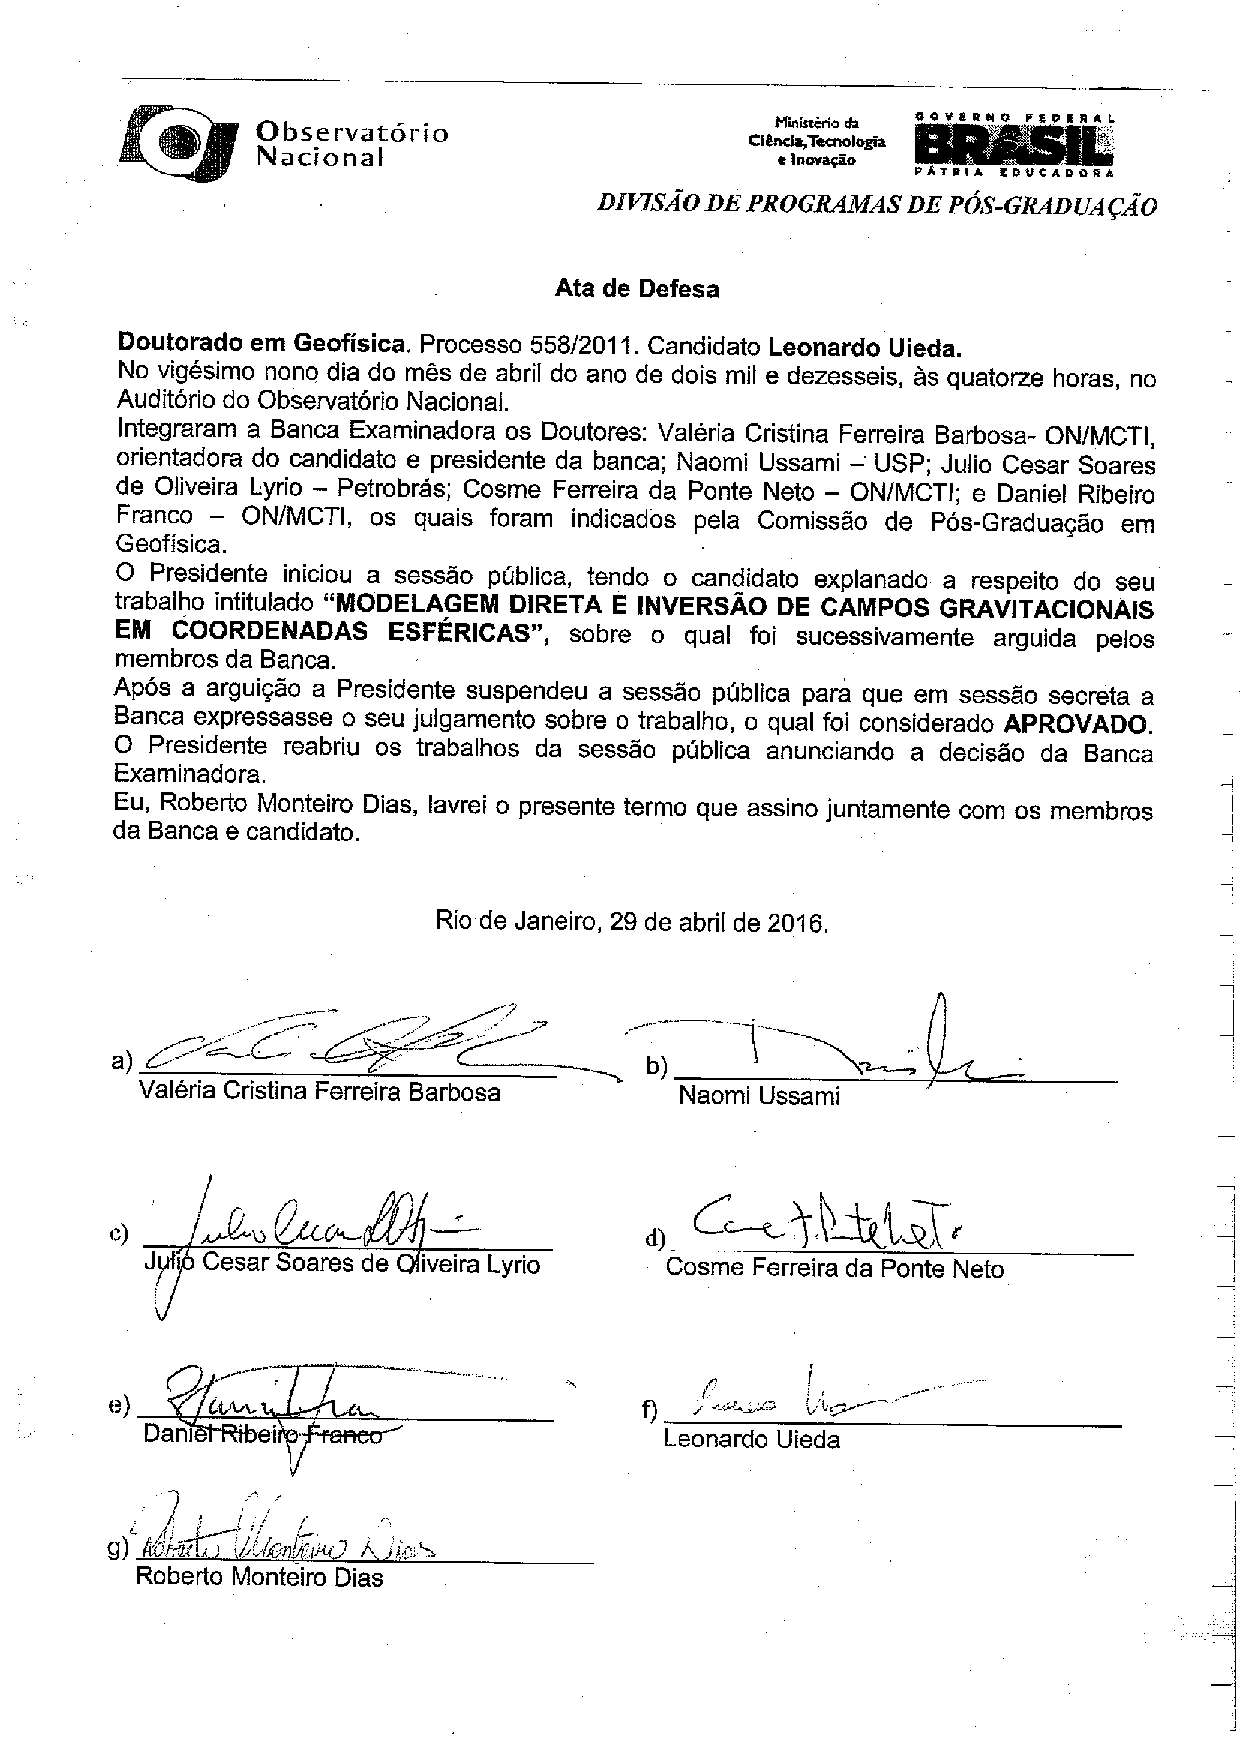
\includepdf[pages={1},pagecommand={\thispagestyle{fancy}},scale=0.8]{comprovantes/edu/ata-defesa-doutorado.pdf}

\includepdf[pages={1},pagecommand={\thispagestyle{fancy}},scale=0.8]{comprovantes/edu/ata-homologacao-doutorado.pdf}

\includepdf[pages={1},pagecommand={\thispagestyle{fancy}\subsubsection{Pós-doutorado na University of Hawaii, E.U.A.}},scale=0.85]{comprovantes/edu/gmt-posdoc.pdf}



\subsection{Atuação profissional}

\includepdf[pages={1},pagecommand={\thispagestyle{fancy}\subsubsection{Professor Assistente, Universidade do Estado do Rio de Janeiro}},scale=0.75]{comprovantes/posse-uerj.pdf}



\subsection{Coordenação de Projetos}


\includepdf[pages={1},pagecommand={\thispagestyle{fancy}\subsubsection{Projeto Qualitec 2014 para o Laboratório de Geofísica de Exploração}},scale=0.75]{comprovantes/qualitec2014.pdf}


\subsection{Revisor de periódicos}



\subsection{Artigos publicados}


\includepdf[pages={1},scale=0.8,pagecommand={\thispagestyle{fancy}\subsubsection{Estimation of the total magnetization direction of approximately spherical bodies}}]{comprovantes/papers/magdir2015.pdf}


\subsection{Trabalhos completos publicados em anais de congressos internacionais}


\subsection{Programas de computador sem registro}


\subsection{Apresentações de trabalho}


\subsection{Participação em bancas}


\subsection{Cursos de curta duração ministrados}



%\includepdf[pages={-},pagecommand={\thispagestyle{plain}}]{comprovantes/email-confirmacao-bolsa-santiago.pdf}

\newpage

\thispagestyle{plain}
\bibliographystyle{gji}
\bibliography{biblio}
\addcontentsline{toc}{section}{Referências}

\end{document}
